\chapter{العطرية والاستبدال العطري المحب للإلكترونات}\label{ch:b2:aromatic-substitution}

يفقد ماء البروم لونه في ثوانٍ حين يُرج مع ألكين،
ولا يفقده إطلاقًا مع البنزين. ومع ذلك يتفاعل البنزين مع البروم حالما تُضاف
كمية قليلة من بروميد الحديد(III) --- والناتج، البروموبنزين، يحتفظ
بحلقته \omterm{def:b2:huckel:aromatic}{العطرية} السداسية: فقد استُبدل هيدروجين واحد، ولم يُضف شيء.
فالحلقات \omterm{def:b2:huckel:aromatic}{العطرية} تخضع للاستبدال لا للإضافة، لأن الإضافة
تضيّع الاستقرار المحسوب في \cref{ch:b2:huckel}. والآلية نفسها
تُنترِت حلقات البنزين وتسلفنها وتؤلكلها وتؤسيلها، 
والمجموعات الموجودة على الحلقة تحدد، بانتظام مدهش، أين تدخل
المجموعة التالية.

\begin{recall}
\Cref{ch:b2:huckel}: \omterm{def:b2:huckel:aromatic}{العطرية} \omterm{def:b2:huckel:delocalisation}{وطاقة اللاتمركز} للبنزين. ومجلد السنة
الأولى: الإضافات المحبة للإلكترونات إلى الألكينات، والتأثيران التحريضي والميزوميري، والمجموعات المانحة 
والساحبة، والكاتيونات الكربونية وإعادة ترتيبها، ومسلّمة هاموند، وأحماض لويس،
ومخططات الطاقة.
\end{recall}

\begin{omfigure}
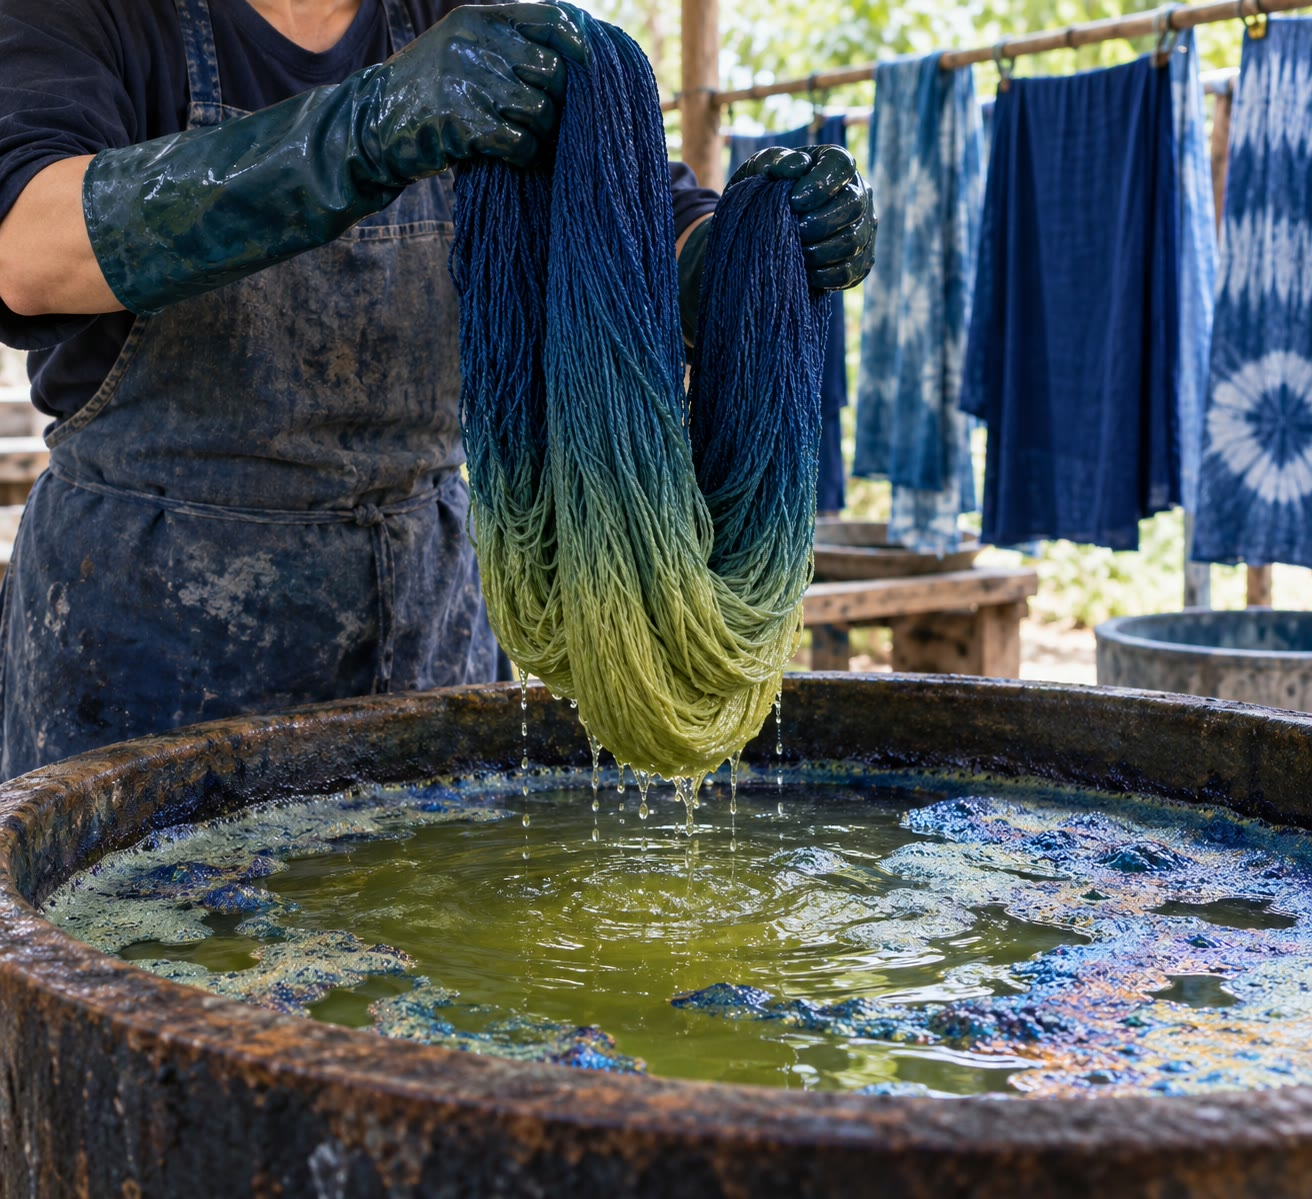
\includegraphics[width=0.55\linewidth]{images/book3/ai/b2-22-indigo-vat-2.jpg}

{\small صباغة الغزل في حوض النيلة (رسم توضيحي). يخرج الغزل من الحوض أصفر مخضرًا، مشبعًا
بالصورة المختزلة الذوابة للصبغة، ثم يصير أزرق في الهواء حين يعيده الأكسجين إلى
النيلة غير الذوابة. والنيلة، مثل معظم الأصباغ، مبنية على حلقات \omterm{def:b2:huckel:aromatic}{عطرية}؛
وقد نشأت صناعة الأصباغ في القرن التاسع عشر من تفاعلات الاستبدال في هذا
الفصل مطبقة على البنزين المستخرج من قطران الفحم.}
\end{omfigure}

\section{استبدال لا إضافة}

\begin{definition}[الأرين]\label{def:b2:aromatic-substitution:arene}
\emph{الأرين}\index{أرين} هيدروكربون يحوي حلقة \omterm{def:b2:huckel:aromatic}{عطرية} واحدة على الأقل، مثل
البنزين، والتولوين (ميثيل بنزين) والنفثالين؛ ومجموعة الأريل (\ce{Ar}) هي أرين نُزع منه
هيدروجين واحد.
\end{definition}

\begin{proposition}[لماذا لا يخضع البنزين للإضافة]\label{prop:b2:aromatic-substitution:no-addition}
الإضافة إلى البنزين تحوّل الحلقة \omterm{def:b2:huckel:aromatic}{العطرية} إلى هكساديين حلقي غير \omterm{def:b2:huckel:aromatic}{عطري} 
وتضيّع معظم الاستقرار \omterm{def:b2:huckel:aromatic}{العطري} البالغ \qty{150}{kJ/mol}؛ أما الاستبدال فيحفظه.
\end{proposition}

\begin{proof}[تعليل]
في \cref{ch:b2:huckel}، وُجد أن هدرجة البنزين إلى الهكسا-1،3-ديين الحلقي
ماصة للحرارة (\qty{+22}{kJ/mol}، من \qty{-206.0}{} و\qty{-227.7}{kJ/mol})، بينما تطلق هدرجة
رابطة مزدوجة عادية \qty{119}{kJ/mol}: فالإضافة الأولى هي الخطوة المكلفة.
وبعد الخطوة المحبة للإلكترونات الأولى، يستطيع الكاتيون المتكوّن إما إضافة محب للنواة، فيبقى
\omterm{def:b2:frontier-orbitals:diels-alder}{ديين} غير \omterm{def:b2:huckel:aromatic}{عطري}، وإما فقد بروتون، فتستعيد الحلقة عطريتها. والمسار الثاني
أكثر مواتاة بكثير.
% ledger: dfh:C6H6_g, dfh:C6H8_g, dfh:C6H10_g, dfh:C6H12_g
\end{proof}

\section{الآلية}

\begin{definition}[الاستبدال العطري المحب للإلكترونات]\label{def:b2:aromatic-substitution:seAr}
\emph{الاستبدال العطري المحب للإلكترونات}\index{استبدال عطري محب للإلكترونات}
يستبدل بهيدروجين من حلقة \omterm{def:b2:huckel:aromatic}{عطرية} محبًا للإلكترونات \ce{E+}. فيرتبط المحب للإلكترونات أولًا
بأحد كربونات الحلقة، معطيًا كاتيونًا يكون فيه ذلك الكربون رباعي الأوجه 
وتتوزع الشحنة الموجبة على الكربونات الخمسة الأخرى: \emph{وسيط ويلاند}\index{وسيط ويلاند}
(أيون أرينيوم). ثم تنزع قاعدة البروتون من الكربون الرباعي الأوجه.
\end{definition}

\begin{proposition}[خطوتان]\label{prop:b2:aromatic-substitution:mechanism}
الخطوة الأولى، التي تهدم \omterm{def:b2:huckel:aromatic}{العطرية}، هي البطيئة؛ أما فقد البروتون،
الذي يعيدها، فسريع.
\end{proposition}

\begin{proof}[تعليل]
\omterm{def:b2:aromatic-substitution:seAr}{وسيط ويلاند} كاتيون كربوني يثبّته اللاتمركز على ثلاثة كربونات
لكنه غير \omterm{def:b2:huckel:aromatic}{عطري}: فهو يقع عاليًا فوق المتفاعلات، وحسب مسلّمة هاموند تكون
الحالة الانتقالية المؤدية إليه قريبة منه في البنية والطاقة. والخطوة الثانية
تنزل إلى ناتج \omterm{def:b2:huckel:aromatic}{عطري}: فحاجزها منخفض.
\end{proof}

\begin{omfigure}
\begin{tikzpicture}
\begin{axis}[width=0.55\linewidth, height=5.4cm, xmin=-0.2, xmax=4.2, ymin=-5.5, ymax=11.5,
  axis x line=bottom, axis y line=left, xtick=\empty, ytick=\empty,
  xlabel={\foreignlanguage{arabic}{إحداثي التفاعل}}, ylabel={\foreignlanguage{arabic}{الطاقة}}, label style={font=\small}, clip=false]
\addplot[omDef, thick] table[x=x, y=sub] {figdata/out/bachelor-2-aromatic-profile.dat};
\addplot[omThm, thick, dashed, restrict x to domain=2:4] table[x=x, y=add] {figdata/out/bachelor-2-aromatic-profile.dat};
\node[font=\scriptsize, anchor=north west] at (axis cs:0.0,-0.6) {\ce{ArH + E+}};
\node[font=\scriptsize, anchor=north] at (axis cs:2,5.7) {ويلاند};
\node[font=\scriptsize, anchor=west, omDef] at (axis cs:4.05,-4.0) {\ce{ArE + H+}};
\node[font=\scriptsize, anchor=west, omThm] at (axis cs:4.05,2.0) {\foreignlanguage{arabic}{ناتج الإضافة}};
\node[font=\scriptsize, anchor=south] at (axis cs:1,10.1) {بطيئة};
\end{axis}
\end{tikzpicture}

{\small مخطط الطاقة \omterm{def:b2:aromatic-substitution:seAr}{لاستبدال عطري محب للإلكترونات}، رسم تخطيطي (وهو نموذج).
للخطوة الأولى، التي تكوّن \omterm{def:b2:aromatic-substitution:seAr}{وسيط ويلاند}، أعلى حاجز. وفقد
بروتون (متصل) يعيد الحلقة \omterm{def:b2:huckel:aromatic}{العطرية}؛ أما إضافة محب للنواة (متقطع) فتترك
ناتجًا فوق المتفاعلات.}
\end{omfigure}

\begin{omfigure}
\setchemfig{atom sep=2em}
\schemestart
\chemfig{HO-\chemabove{N}{\scriptstyle +}(=[1]O)-[7]\chemabove{O}{\scriptstyle -}} \+ \chemfig{H_2SO_4}
\arrow{<=>}
\chemfig{O=N^{+}=O} \+ \chemfig{HSO_4^{-}} \+ \chemfig{H_2O}
\schemestop

\medskip
\begin{tikzpicture}[font=\small, >={Stealth}]
\tikzset{pics/whel/.style n args={4}{code={
    \foreach \k in {0,...,5} \draw[thick] ({90+60*\k}:0.7) -- ({150+60*\k}:0.7);
    \foreach \k in {#1} \draw[thick] ($({90+60*\k}:0.56)!0.18!({150+60*\k}:0.56)$) -- ($({90+60*\k}:0.56)!0.82!({150+60*\k}:0.56)$);
    \ifnum#2>-1 \node[font=\scriptsize] at ({90+60*#2}:0.36) {$+$};\fi
    \draw[thick] (270:0.7) -- ++(-125:0.42) node[anchor=north east, inner sep=1pt, font=\scriptsize] {H};
    \draw[thick] (270:0.7) -- ++(-55:0.42) node[anchor=north west, inner sep=1pt, font=\scriptsize] {#4};
    \if\relax\detokenize{#3}\relax\else
      \draw[thick] (90:0.7) -- (90:1.1) node[anchor=south, inner sep=1pt, font=\scriptsize] {#3};\fi
  }}}
  \foreach \k in {0,...,5} \draw[thick] ({90+60*\k}:0.7) -- ({150+60*\k}:0.7);
  \foreach \k in {0,2,4} \draw[thick] ($({90+60*\k}:0.56)!0.18!({150+60*\k}:0.56)$) -- ($({90+60*\k}:0.56)!0.82!({150+60*\k}:0.56)$);
  \node at (1.3,0) {$+$};
  \node at (2.0,0) {\ce{NO2+}};
  \draw[->, thick] (2.6,0) -- (3.8,0) node[midway, above, font=\scriptsize] {بطيئة};
  \pic at (4.7,0.1) {whel={1,4}{0}{}{\ce{NO2}}};
  \draw[->, thick] (5.6,0) -- (6.8,0) node[midway, above, font=\scriptsize] {سريعة} node[midway, below, font=\scriptsize] {$-$\ce{H+}};
  \begin{scope}[xshift=7.7cm]
    \foreach \k in {0,...,5} \draw[thick] ({90+60*\k}:0.7) -- ({150+60*\k}:0.7);
    \foreach \k in {0,2,4} \draw[thick] ($({90+60*\k}:0.56)!0.18!({150+60*\k}:0.56)$) -- ($({90+60*\k}:0.56)!0.82!({150+60*\k}:0.56)$);
    \draw[thick] (270:0.7) -- (270:1.1) node[anchor=north, font=\scriptsize] {\ce{NO2}};
  \end{scope}
\end{tikzpicture}
\par\vspace{6pt}

{\small نترتة البنزين. يبرتن حمض الكبريتيك حمض النتريك، الذي يفقد الماء: فيكون
أيون النترونيوم \ce{NO2+} هو المحب للإلكترونات. ويرتبط بأحد الكربونات (بطيئة)، معطيًا
\omterm{def:b2:aromatic-substitution:seAr}{وسيط ويلاند}، الذي تتوزع شحنته الموجبة على الحلقة؛ ثم يعطي فقد بروتون
(سريع) النتروبنزين.}
\end{omfigure}

\section{التفاعلات}

\paragraph{الهلجنة.} البروم أو الكلور وحده محب للإلكترونات أضعف من اللازم؛ فحمض لويس
(\ce{FeBr3}، \ce{AlCl3}) يستقطب الهالوجين بالارتباط بإحدى ذرتيه، فتهاجم ذرة
البروم الخارجية الحلقة.

\paragraph{النترتة.} يعطي خليط من حمضي النتريك والكبريتيك المركزين (أعلاه)
أيون النترونيوم.

\paragraph{السلفنة.} يعطي حمض الكبريتيك المدخن (\ce{SO3} في \ce{H2SO4}) حمض البنزين سلفونيك.
والتفاعل عكوس: فتسخين حمض السلفونيك في حمض مائي مخفف يزيل
مجموعة \ce{SO3H} من جديد، مما يجعلها مجموعة حجب مؤقتة مفيدة.

\begin{definition}[تفاعلات فريدل--كرافتس]\label{def:b2:aromatic-substitution:friedel-crafts}
\emph{ألكلة فريدل--كرافتس}\index{ألكلة فريدل--كرافتس} تربط مجموعة ألكيل
بحلقة \omterm{def:b2:huckel:aromatic}{عطرية} انطلاقًا من ألكان مهلجن وحمض لويس (\ce{AlCl3}). 
و\emph{أسيلة فريدل--كرافتس}\index{أسيلة فريدل--كرافتس} تربط مجموعة أسيل
\ce{RCO} انطلاقًا من كلوريد أسيل و\ce{AlCl3}، عبر \emph{أيون الأسيليوم}\index{أيون الأسيليوم}
\ce{R-C#O+}، فتعطي كيتونًا أريليًا.
\end{definition}

\begin{proposition}[حدود تفاعلات فريدل--كرافتس]\label{prop:b2:aromatic-substitution:friedel-crafts-limits}
تعاني \omterm{def:b2:aromatic-substitution:friedel-crafts}{ألكلة فريدل--كرافتس} من إعادة ترتيب الكاتيون الكربوني ومن
تعدد الألكلة؛ أما الأسيلة فتتوقف بعد استبدال واحد، ولا تعطي إعادة ترتيب، وتحتاج إلى
مكافئ واحد على الأقل من \ce{AlCl3}. ولا يصلح أي منهما على حلقة تحمل \omterm{def:b2:aromatic-substitution:directing}{مجموعة
مثبطة} بقوة.
\end{proposition}

\begin{proof}[تعليل]
المحب للإلكترونات المؤلكِل كاتيون كربوني (أو معقد مستقطب يسلك سلوكه)،
يعاد ترتيبه إلى كاتيون أكثر استقرارًا بانتقال هيدريد أو ألكيل: فيعطي 1-كلوروبروبان
إيزوبروبيل بنزين في معظمه. ومجموعة الألكيل تنشط الحلقة (الفقرة التالية)، فيتفاعل الناتج
أسرع من البنزين ويؤلكل من جديد. أما \omterm{def:b2:aromatic-substitution:friedel-crafts}{أيون الأسيليوم} فيثبّته
الرنين (\ce{R-C+=O} $\leftrightarrow$ \ce{R-C#O+}) ولا يعاد ترتيبه؛ ومجموعة الأسيل
تثبّط الحلقة، فلا يتفاعل الناتج أكثر؛ والكيتون المتكوّن يرتبط
بالمركب \ce{AlCl3} عبر أكسجينه، فينتزع الحفاز من التفاعل: فيُستهلك مكافئ
واحد. والحلقة المثبطة بقوة محب للنواة أفقر من أن تتفاعل مع هذه المحبات للإلكترونات الضعيفة.
\end{proof}

\section{آثار البدائل}

\begin{definition}[المجموعات الموجِّهة]\label{def:b2:aromatic-substitution:directing}
يكون البديل على حلقة بنزين \emph{مجموعة منشطة}\index{مجموعة منشطة} إذا كانت
الحلقة تتفاعل أسرع من البنزين، و\emph{مجموعة مثبطة}\index{مجموعة مثبطة} إذا كانت
تتفاعل أبطأ. ويكون \emph{موجِّهًا أورثو/بارا}\index{موجه أورثو/بارا} إذا دخلت المجموعة
الجديدة أساسًا في المواضع المجاورة له والمقابلة له، و\emph{موجِّهًا
ميتا}\index{موجه ميتا} إذا دخلت أساسًا في المواضع التي تبعد عنه موضعًا واحدًا.
\end{definition}

\begin{proposition}[المانحات والساحبات]\label{prop:b2:aromatic-substitution:directing}
المجموعات التي تمنح الحلقة إلكترونات بالتأثير الميزوميري (\ce{-OH}، \ce{-OCH3}، \ce{-NH2}،
\ce{-NHCOCH3}) أو بالتأثير التحريضي \omterm{def:b2:fragment-orbitals:hyperconjugation}{وفرط الاقتران} (الألكيلات) تنشط الحلقة وتوجّه
إلى أورثو/بارا. والمجموعات الساحبة للإلكترونات بالتأثير الميزوميري (\ce{-NO2}، \ce{-CN}، \ce{-COR}،
\ce{-COOH}، \ce{-SO3H}) تثبطها وتوجّه إلى ميتا.
\end{proposition}

\begin{proof}
قارن وسائط ويلاند. ففي الهجوم أورثو أو بارا بالنسبة إلى بديل G، تضع إحدى
بنى الرنين الثلاث الشحنة الموجبة على الكربون الحامل للمجموعة G؛ وفي الهجوم ميتا،
لا تضعها أي منها. والمانح G (زوج حر على O أو N) يثبّت شحنة موجبة على الكربون المرتبط
به، مضيفًا بنية رنين رابعة يكون فيها لكل ذرة ثمانية: فتنخفض الوسائط أورثو
وبارا، وحسب مسلّمة هاموند تنخفض كذلك الحالات الانتقالية
المؤدية إليها. أما الساحب G فيزعزع استقرار الشحنة الموجبة على كربونه: فترتفع الوسائط أورثو وبارا،
ويكون الهجوم ميتا، الذي يتجنب تلك البنية، الأقل
إعاقة، وإن كان أبطأ منه على البنزين.
\end{proof}

\begin{omfigure}
\begin{tikzpicture}[font=\small]
\tikzset{pics/whel/.style n args={4}{code={
    \foreach \k in {0,...,5} \draw[thick] ({90+60*\k}:0.7) -- ({150+60*\k}:0.7);
    \foreach \k in {#1} \draw[thick] ($({90+60*\k}:0.56)!0.18!({150+60*\k}:0.56)$) -- ($({90+60*\k}:0.56)!0.82!({150+60*\k}:0.56)$);
    \ifnum#2>-1 \node[font=\scriptsize] at ({90+60*#2}:0.36) {$+$};\fi
    \draw[thick] (270:0.7) -- ++(-125:0.42) node[anchor=north east, inner sep=1pt, font=\scriptsize] {H};
    \draw[thick] (270:0.7) -- ++(-55:0.42) node[anchor=north west, inner sep=1pt, font=\scriptsize] {#4};
    \if\relax\detokenize{#3}\relax\else
      \draw[thick] (90:0.7) -- (90:1.1) node[anchor=south, inner sep=1pt, font=\scriptsize] {#3};\fi
  }}}
  \node[anchor=east] at (-1.0,0) {\foreignlanguage{arabic}{ميثوكسي، هجوم بارا:}};
  \pic at (0,0) {whel={1,4}{0}{\ce{OCH3}}{E}};
  \node at (1.25,0.1) {$\leftrightarrow$};
  \begin{scope}[xshift=2.5cm]
    \foreach \k in {0,...,5} \draw[thick] ({90+60*\k}:0.7) -- ({150+60*\k}:0.7);
    \foreach \k in {1,4} \draw[thick] ($({90+60*\k}:0.56)!0.18!({150+60*\k}:0.56)$) -- ($({90+60*\k}:0.56)!0.82!({150+60*\k}:0.56)$);
    \draw[thick] (-0.06,0.7) -- (-0.06,1.1); \draw[thick] (0.06,0.7) -- (0.06,1.1);
    \node[anchor=south, inner sep=1pt, font=\scriptsize] at (0,1.1) {$\overset{+}{\mathrm O}\mathrm{CH_3}$};
    \draw[thick] (270:0.7) -- ++(-125:0.42) node[anchor=north east, inner sep=1pt, font=\scriptsize] {H};
    \draw[thick] (270:0.7) -- ++(-55:0.42) node[anchor=north west, inner sep=1pt, font=\scriptsize] {E};
  \end{scope}
  \node[anchor=west, font=\scriptsize] at (3.4,0) {\foreignlanguage{arabic}{بنية إضافية، لكل ذرة فيها ثمانية}};
  \begin{scope}[yshift=-3.5cm]
    \node[anchor=east] at (-1.0,0) {\foreignlanguage{arabic}{نترو، هجوم بارا:}};
    \pic at (0,0) {whel={1,4}{0}{\ce{NO2}}{E}};
    \node[anchor=west, font=\scriptsize] at (1.0,0) {\foreignlanguage{arabic}{شحنة موجبة على الكربون الحامل للمجموعة الساحبة}};
  \end{scope}
\end{tikzpicture}

{\small وسائط ويلاند للهجوم بارا بالنسبة إلى بديل. مع الميثوكسي، يشارك زوج حر
للأكسجين في حمل الشحنة الموجبة (بنية رنين إضافية، لكل ذراتها ثمانية):
فيستقر الوسيط، ويكون البديل منشطًا وموجّهًا أورثو/بارا. ومع
النترو، تضع إحدى البنى الشحنة الموجبة على الكربون الحامل للمجموعة الساحبة
للإلكترونات: فيضطرب استقرار الوسيط، ويتجه الهجوم إلى ميتا.}
\end{omfigure}

\begin{proposition}[الهالوجينات]\label{prop:b2:aromatic-substitution:halogens}
بدائل الهالوجين تثبط الحلقة لكنها توجّه إلى أورثو/بارا.
\end{proposition}

\begin{proof}[تعليل]
سحبها التحريضي (الكهرسلبية) يخفض الكثافة الإلكترونية للحلقة كلها
ويبطئ كل هجوم: فهي مثبطة. لكن زوجًا حرًا للهالوجين يستطيع مع ذلك المشاركة في حمل
الشحنة الموجبة لوسيطي ويلاند أورثو وبارا، وهو ما لا يستطيعه الوسيط ميتا:
فمن بين الهجمات الأبطأ، يبقى أورثو وبارا الأقل بطئًا.
\end{proof}

\section{البنزينات المتعددة الاستبدال}

\begin{method}[التنبؤ بموضع الاستبدال]\label{met:b2:aromatic-substitution:predict-position}
\begin{enumerate}
  \item علّم لكل بديل المواضع التي يفضّلها (أورثو/بارا أو ميتا).
  \item إذا اتفقت، فاز ذلك الموضع. وإذا اختلفت، حسم المنشط الأقوى
        (\babelsublr{\ce{-NH2},~\ce{-OH}~$>$~\ce{-OCH3}~$>$~\ce{-NHCOCH3}~$>$~\foreignlanguage{arabic}{ألكيل}~$>$~\foreignlanguage{arabic}{هالوجين}}).
  \item تجنب الموضع الواقع بين بديلين في علاقة 1،3 (معاق)، 
        وتوقع بارا أكثر من أورثو حين تكون المجموعات ضخمة.
\end{enumerate}
\end{method}

\begin{method}[تخطيط تخليق عطري]\label{met:b2:aromatic-substitution:plan-aromatic}
\begin{enumerate}
  \item اختر ترتيب الخطوات بحيث توجّه كل مجموعة موجودة المجموعة التالية
        حيث يُراد: لتحضير 3-برومونتروبنزين، نترِت أولًا (موجّه ميتا)، ثم
        برومن؛ ولتحضير 4-برومونتروبنزين، برومن أولًا.
  \item استعمل مجموعات قابلة للتحويل: يمكن اختزال مجموعة أسيل (ميتا) إلى ألكيل (أورثو/بارا)؛
        واختزال مجموعة نترو (ميتا) إلى أمين (أورثو/بارا)؛ وأكسدة ألكيل إلى
        \ce{-COOH} (ميتا).
  \item احجب موضعًا بالمجموعة \ce{-SO3H} وأزلها في النهاية.
  \item روّض منشطًا قويًا: يؤسَّل الأمين (\ce{-NHCOCH3}) قبل النترتة أو
        الهلجنة، ثم يُحرَّر من جديد.
\end{enumerate}
\end{method}

\begin{history}[فريدل وكرافتس]
\begin{minipage}[t]{0.18\linewidth}
\vspace{0pt}
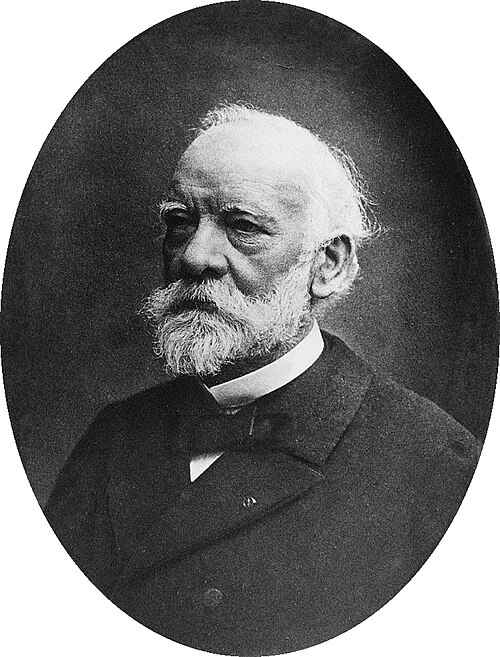
\includegraphics[width=\linewidth]{images/book3/friedel.jpg}
\end{minipage}\hspace{0.02\linewidth}%
\begin{minipage}[t]{0.18\linewidth}
\vspace{0pt}
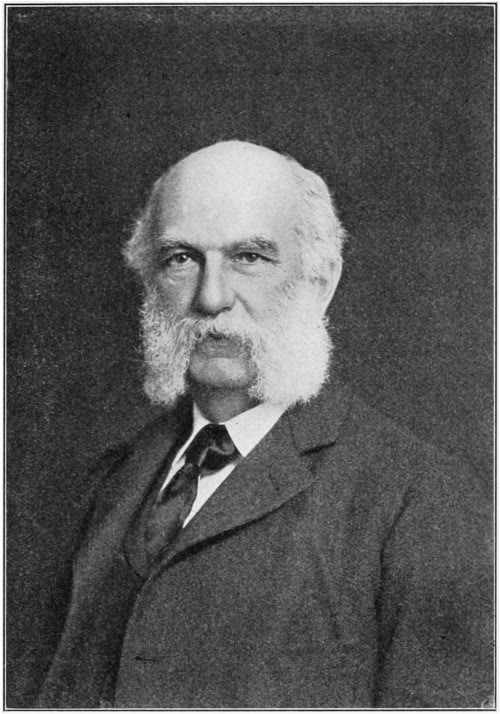
\includegraphics[width=\linewidth]{images/book3/crafts.jpg}
\end{minipage}\hfill
\begin{minipage}[t]{0.58\linewidth}
\vspace{0pt}
في سنة 1877 وجد شارل فريدل وجيمس ميسون كرافتس، وهما يعملان معًا في باريس، أن
كلوريد الألومنيوم يجعل الألكانات المهلجنة وكلوريدات الأسيل تتفاعل مع البنزين. وصارت
تفاعلاتهما الطريقة المعيارية لربط مجموعات كربونية بالحلقات \omterm{def:b2:huckel:aromatic}{العطرية}، وامتد حفز
أحماض لويس الذي اكتشفاه إلى ما هو أبعد من ذلك بكثير. (صورتان شخصيتان: فريدل، تسعينيات القرن التاسع عشر؛ وكرافتس، من
مجلة «بوبيولار ساينس مانثلي»، 1900؛ ملكية عامة، ويكيميديا كومنز.)
\end{minipage}
\end{history}

\begin{safety}{\ghs[5mm]{GHS02}\,\ghs[5mm]{GHS05}\,\ghs[5mm]{GHS06}\,\ghs[5mm]{GHS08}}
البنزين مسرطن ويُستبدل به التولوين أو أرينات أخرى حيثما أمكن.
وحمضا النتريك والكبريتيك المركزان أكّالان وخليط النترتة مؤكسد
بشدة؛ فيُبرَّد ويُضاف \omterm{def:b2:aromatic-substitution:arene}{الأرين} ببطء، لأن النترتات ناشرة للحرارة.
والبروم شديد السمية وأكّال؛ وكلوريد الألومنيوم يتفاعل بعنف مع الماء. والنتروأرينات
سامة.
% ledger: ghs:benzene, ghs:toluene, ghs:HNO3, ghs:H2SO4, ghs:Br2, ghs:AlCl3, ghs:nitrotoluene-4
\end{safety}

\section{تمارين}

\begin{exercise}[$\star$]\label{exo:b2:aromatic-substitution:1}
اكتب تكوّن أيون النترونيوم من حمض النتريك وحمض الكبريتيك.
\end{exercise}

\begin{exercise}[$\star$]\label{exo:b2:aromatic-substitution:2}
أعطِ النواتج الرئيسية لبرومنة (\ce{Br2}، \ce{FeBr3}) التولوين 
والنتروبنزين.
\end{exercise}

\begin{exercise}[$\star$]\label{exo:b2:aromatic-substitution:3}
صنّف إلى منشط أو مثبط، وأورثو/بارا أو ميتا: \ce{-CH3}، \ce{-OH}، \ce{-Cl}،
\ce{-NO2}، \ce{-COCH3}، \ce{-NHCOCH3}.
\end{exercise}

\begin{exercise}[$\star$]\label{exo:b2:aromatic-substitution:4}
أعطِ ناتج البنزين مع كلوريد الإيثانويل وكلوريد الألومنيوم.
\end{exercise}

\begin{exercise}[$\star\star$]\label{exo:b2:aromatic-substitution:5}
يعطي البنزين و1-كلوروبروبان مع \ce{AlCl3} إيزوبروبيل بنزين أساسًا. فسّر، وأعطِ
طريقًا من خطوتين إلى بروبيل بنزين.
\end{exercise}

\begin{exercise}[$\star\star$]\label{exo:b2:aromatic-substitution:6}
يزيل الفينول لون ماء البروم فورًا، دون حفاز، معطيًا
2،4،6-ثلاثي بروموفينول. فسّر.
\end{exercise}

\begin{exercise}[$\star\star$]\label{exo:b2:aromatic-substitution:7}
أعطِ طرائق تخليق 3-برومونتروبنزين و4-برومونتروبنزين انطلاقًا من البنزين.
\end{exercise}

\begin{exercise}[$\star\star$]\label{exo:b2:aromatic-substitution:8}
تُنترَت الأنيلين نترتة رديئة (أكسدة، وناتج ميتا)، لكن الأسيتانيليد يعطي أساسًا
4-نتروأسيتانيليد. فسّر الحقيقتين كلتيهما.
\end{exercise}

\begin{exercise}[$\star\star$]\label{exo:b2:aromatic-substitution:9}
بيّن كيف يمكن استعمال مجموعة حمض السلفونيك لتحضير 2-بروموتولوين خاليًا من متماكبه بارا.
\end{exercise}

\begin{exercise}[$\star\star\star$]\label{exo:b2:aromatic-substitution:10}
أين تحدث نترتة 4-ميثيل أنيسول (4-ميثوكسي تولوين)؟ فسّر بالمجموعتين
الموجِّهتين.
\end{exercise}

\begin{exercise}[$\star\star\star$]\label{exo:b2:aromatic-substitution:11}
يُصنع 2،4،6-ثلاثي نتروتولوين بثلاث نترتات متتالية للتولوين، كل منها في ظروف أقسى
من سابقتها. فسّر السبب.
\end{exercise}

\begin{exercise}[$\star\star\star$]\label{exo:b2:aromatic-substitution:12}
اقترح تخليقًا لحمض 4-نتروبنزويك انطلاقًا من التولوين، ولحمض 3-نتروبنزويك.
\end{exercise}

\section{مسألة: نترتة التولوين}

\begin{problem}[{مسألة نهاية الأسبوع --- أيون النترونيوم وآلية النترتة، 
والمواضع أورثو وميتا وبارا للتولوين مقارنة بالنسبة الإحصائية، وفصل
المتماكبات، وموازنة كتلية}]
\label{pb:b2:aromatic-substitution:1}
المعطيات: درجات الانصهار: 2-نتروتولوين \qty{-10}{\degreeCelsius}، و3-نتروتولوين
\qty{16}{\degreeCelsius}، و4-نتروتولوين \qty{52}{\degreeCelsius}. ومعطيات تمرين لتجربة:
\qty{100}{g} من التولوين، \omterm{def:b2:continuous-reactors:conversion}{والتحويل} 90~\%، وتوزيع المتماكبات 58~\% أورثو، و4~\% ميتا، 
و38~\% بارا. والكتل المولية (\unit{g/mol}): C 12.011، H 1.008، N 14.007، O 15.999.
% ledger: mp:2-nitrotoluene, mp:3-nitrotoluene, mp:4-nitrotoluene, aw:C, aw:H, aw:N, aw:O

\medskip
\noindent\textbf{الجزء الأول --- المحب للإلكترونات والآلية.}
\begin{enumerate}
  \item اكتب تكوّن أيون النترونيوم.
  \item ارسم بنية لويس له وأعطِ شكله.
  \item اكتب هجوم \ce{NO2+} على التولوين في الموضع بارا بالنسبة إلى الميثيل.
  \item ارسم بنى الرنين الثلاث \omterm{def:b2:aromatic-substitution:seAr}{لوسيط ويلاند} بارا.
  \item أي الخطوات محددة للسرعة؟
  \item ما الذي ينزع البروتون في الخطوة الثانية؟
\end{enumerate}

\medskip
\noindent\textbf{الجزء الثاني --- المواضع الثلاثة.}
\begin{enumerate}[resume]
  \item كم موضعًا أورثو وميتا وبارا في التولوين؟
  \item ما النسبة التي يعطيها هجوم عشوائي؟
  \item ارسم \omterm{def:b2:aromatic-substitution:seAr}{وسيط ويلاند} ميتا وفسّر لماذا هو الأقل استقرارًا.
  \item كيف تثبّت مجموعة الميثيل الوسيطين أورثو وبارا؟
  \item قارن النسبة المشاهدة بالنسبة الإحصائية: أي المواضع مفضّلة؟
  \item قارن المردود لكل موضع عند أورثو (نصف النسبة المئوية لأورثو) وعند بارا.
        اقترح سببًا للفرق.
  \item هل تُنترَت التولوين أسرع من البنزين أم أبطأ؟
\end{enumerate}

\medskip
\noindent\textbf{الجزء الثالث --- الفصل.}
\begin{enumerate}[resume]
  \item أي المتماكبات صلب في درجة حرارة الغرفة؟
  \item اقترح طريقة لعزله من الخليط بالتبريد.
  \item لماذا يحابي التناظر درجةَ انصهار مرتفعة؟
  \item كيف يمكن بعد ذلك فصل المتماكبين أورثو وميتا؟
  \item لماذا يصعب فصل هذه المتماكبات بالتقطير البسيط؟
\end{enumerate}

\medskip
\noindent\textbf{الجزء الرابع --- الموازنة الكتلية.}
\begin{enumerate}[resume]
  \item احسب الكتلة المولية للتولوين وللنتروتولوين.
  \item احسب كمية التولوين وكمية النتروتولوين المتكوّن.
  \item احسب كتل المتماكبات الثلاثة.
  \item ما التفاعل الإضافي الذي يجب تجنبه بالتبريد وبعدم استعمال فائض من الحمض؟
  \item كيف تحضّر حمض 4-نتروبنزويك من المتماكب بارا؟
  \item اذكر كتلة 4-نتروتولوين الناتجة من \qty{100}{g} من التولوين في هذه التجربة.
\end{enumerate}
\end{problem}
